\documentclass[12pt]{article}

\usepackage{geometry, subfiles}
\usepackage{amsmath, amssymb}
\usepackage{booktabs, longtable, siunitx}
\usepackage{graphicx}
\graphicspath{{/Users/wonjun/Dropbox/Emory/ECON771_health2/assignments/assignment2/output/}}

\title{Assignment 2}
\author{Wonjun Choi}

\begin{document}
\maketitle
	\begin{itemize}
		\item[1.] Table 1 presents the summary statistics of total spending, the number of claims, and the number of patients for each physicians over the period over 2012 to 2017.
		\subfile{../output/tab_sumstat}
		
		
		\item[2.] The upper line is the trend of unintegrated physicians, and the bottom line is of integrated physicians. The total number of claims of unintegrated physicians begins to increase after the price shock is fully implemented, while it remains in the similar level for integrated physicians. The figure is rescaled to be put in the right place.
		\begin{figure} [ht]
			\centering
			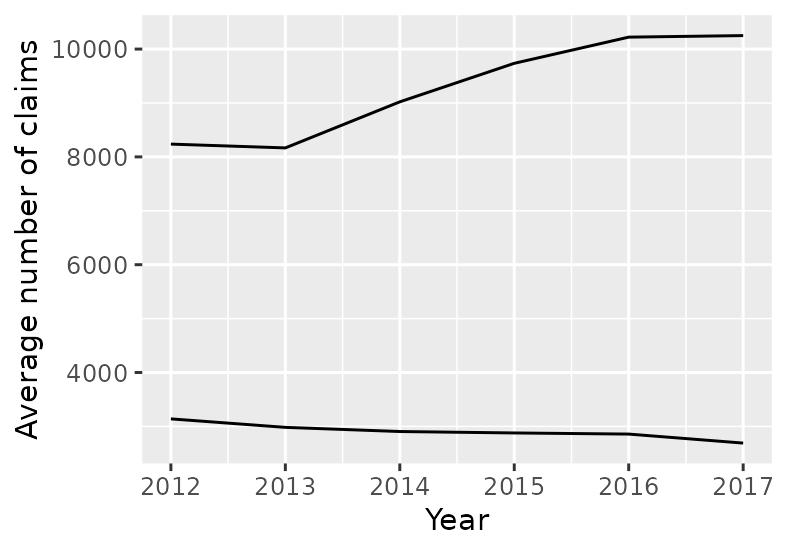
\includegraphics[scale=0.2]{fig_claim_by_int.jpg}
			\caption{Trend of total number of claims by integration status}
		\end{figure}
		
		\item[3.] Table 2 contains the OLS result of regressing the total number of claims on integration status. I added physician level and year level fixed effects in the regression. The standard error was clustered in physician level. The result suggests that the integrated physicians makes 0.4\% less claims than the unintegrated physicians.
		
		\begin{table} [ht]
	    \subfile{../output/tab_twfe_claim_int}
	    \caption{OLS}
		\end{table}

	    	    		
		\item[4.] If the treatment variable $INT$ is correlated with unobserved variables, the coefficient can be biased. We assume hypothetical correlation and see how the coefficient can change in several scenarios following Altonji et al. (2005) and Oster (2019). We consider the following construction.
		\begin{eqnarray*}
			\delta^* \approx \hat{\delta}_{D,x_1} - \rho \times [\hat{\delta}_D - \hat{\delta}_{D,x_1}] \times \frac{R_{max}^2 - R_{D,x_1}^2}{R_{D,x_1}^2 - R_D^2} \xrightarrow{p} \delta
		\end{eqnarray*}
	where $x_1$ is a control variables (fixed effects) and $\hat{\delta}_X$ and $R^2_X$ indicates the treatment effect and $R^2$ in the regression when a vector $X$ is used as a regressor. $R_{max}^2$ is a hypothetical goodness-of-fit $R^2$ in a scenario where we were able to observe unobserved variables. $R_{max}^2 =1$ indicates the situation where we can observe every variables that determines the outcome. $\rho$ is the hypothetical correlation between the treatment variable and the unobservables. I think I included the rownames in R code, but it somehow disappeared.
	
		\begin{tiny}
    	    \subfile{../output/tab_AET}
		\end{tiny}
    
    	Table 3 displays the hypothetical 95\% confidence intervals in each scenarios with $\rho \in \{-1, -0.5, 0, 0.5, 1\}$ and $R_{max}^2 \in \{0.5, 0.6, 0.7, 0.8, 0.9, 1\}$. Since the original $R^2_{D,x_1}$ was already $0.91$, the results of $R_{max}^2 \le 0.9$ is omitted. The treatment effect was significantly negative in every scenarios although the magnitude varied.
    	
    	\item[5.] The treatment variable $INT$ can be endogenous if the number of claims is under consideration in the decision of whether to merge. To estimate the true treatment effect, I use an exogenous price change as an instruement of the treatment.
	\begin{table}[h]
    		\subfile{../output/tab_iv}
    		\caption{2SLS}
    	\end{table}
    
        Table 4 presents the 2SLS results. The treatment effect coefficient was -4.72.
				
		\item[6.] $INT$ can reflect some effect from the unobserved variables. We isolate the treatment effect from the other effects by implementing Durbin-Wu-Hausman test with an augmented regression
		\begin{eqnarray*}
			y_{it} = \delta INT_{it} + \gamma_i + \gamma_t + \kappa \hat{\nu} + \epsilon_{it}
		\end{eqnarray*}
	where $\hat{\nu} = INT_{it} - \hat{INT}_{it}$ is a orthogonalized treatment variable that captures the effect of $INT$ other than the treatment effect.
		\begin{table} [ht]
		\subfile{../output/tab_DWHtest}
		\caption{DWH test}
	\end{table}

    Table 5 displays the result of DWH test. From the coefficient of $INTres$, we can see the treatment variable indeed captures some other effects if it is not instrumented. The result implies that integration actually decreases the number of claims, but  there are some systematic difference in integrated and unintegrated physicians (I am not sure).
		
		\item[7.] If the instrument variable does not sufficiently explains the treatment variable, the IV results might be unreliable. We suggest 2 confidence intervals that takes the weak instruemnt problem into account.
		\subfile{../output/tab_ci}
		
		Table 6 shows the confidence intervals. They were not that different from the previous 2SLS estimator. Actually, the first stage F statistic was over 4000, so in our exercise the instrument has a sufficient explanation power.
			
		\item[8.] Our instrument variable is a function of an exogenous price shock and physican characteristics. However, physician characteristics can be possibly endogenous. To eliminate the possible endogeneity, Borusyak and Hull (2021) working paper suggested recentering the instrument variable with simulated pseudo instruments. See Question 8 of HW2 for detail.
		
		\begin{table}[ht]
    		\subfile{../output/tab_BH}
    		\caption{Borusyak and Hull (2021)}
		\end{table}

		Table 7 shows the estimation results with the recentered instrument. The treatment effect was significantly smaller than the original 2SLS estimates.

		\item[9.] In this exercise, we did only one main estimation (2SLS). All of the other things were auxiliary analysis. The results consistently indicates integration and the number of claims has a negative relationship, but the magnitude varies especially in Borusyak and Hull's approach suggesting that the instrument might be able to polished more.
		
		\item[10.] I think I could have learn more about practical issues of IV, which was so fun, if I started the assignment earlier. I thought I would be able to start earlier, but I was ignorant of the fact that the semester usually gets busier as time goes by. Also, the data work is quite overwhelming. I can't imagine doing this without the guidance code. But I think I learned a lot, anyway. Researchers are great people.
		
	\end{itemize}
\end{document}